\documentclass[]{article}
\usepackage[]{graphicx} 
\usepackage[utf8]{inputenc} 
\usepackage[OT1]{fontenc} 
\usepackage[]{subcaption} 
\usepackage{simplewick}
\usepackage{caption}
\usepackage{amsmath}
\usepackage[]{mathtools} 
\usepackage[]{amssymb} 
\usepackage{prettyref}
\newrefformat{fig}{Figure~[\ref{#1}]}

\begin{document}

\title{Supervised Learning of Behaviors}
\author{Felipe Glicério Gomes Marcelino}
\date{18 April 2020}
\maketitle

\section{Notes}%
\label{sec:Notes}

\subsection*{Slide 3}%
\label{sub:Slide 3}
\begin{enumerate}
    \item Definition of sequential decision problems
    \item Imitation Learning: supervised learning for decision making
        \begin{itemize}
            \item Does direct imitation work?
            \item How can we make it work more often
        \end{itemize}
    \item A little bit of theory
    \item Case studies of recent work in \textbf{deep imitation learning}
    \item Goals:
        \begin{itemize}
            \item Understand definitions \& notation
            \item Understand basic limitation learning algorithms
            \item Understand tools for theoretical analysis
        \end{itemize}
\end{enumerate}

\subsection*{Slide 4 - 5}%
\label{sub:Slide 4 - 5}
\par Terminology \& Notation
\begin{itemize}
    \item $\textbf{a}_{t}$ or $\textbf{u}_{t} $ - action - Output of the classifier
    \item $\textbf{s}_{t}$ or $\textbf{x}_{t} $ - state - \textit{Explained below} 
    \item $\textbf{o}_{t}$ - observation - Image
    \item $\pi_{\theta}(a|b)$ - policy - Distributions over actions given the observation 
    \item $\theta $ is the parameters of the
        model
    \item \textit{t }- time step
\end{itemize}

\par The action can be discrete like:
\begin{enumerate}
    \item Run Away
    \item Ignore
    \item Pet
\end{enumerate}
\par Or can be continues: The direction do you want to run when you see the pictures. It can be achieve using
multivariate normal distributions. 
\par  Deterministic policy - As simply a conditional distribution that  outputs a Dirac Delta over just a single action
- So one action has probability one and everything else has probability zero.
\par Some policies is dependent of states and not observation.  The difference between states and observations is: An
observation that is possible to see. For instance, image pixels. On the other hand, the state is a representation of
this image. For example, the image of Cheetah can be represented as physical state: velocity, position, orientation,
composition of Cheetah body and etc. The states fully describe everything that is going on in the world whereas the
observations can be indistinguishable to someone but has different states between them. 

\par Or can be continuous: The direction do you want to run when you see the pictures. The action can be moduled using multivariate normal distributions.

\par Or can be continuous: The direction do you want to run when you see the pictures. The action uses multivariate normal distributions as a model, for example.

\par Deterministic policy - As simple a conditional distribution that outputs a Dirac Delta over just a single action - So one action has probability one, and everything else has probability zero.
\par 
\begin{itemize}
    \item Some policies are dependent on states and not observation. The difference between states and observations is: 
        An observation that is possible to see. For instance, image pixels. On the other hand, the state is a representation of this image. For example, the image of a cheetah represented as a physical state: velocity, position, orientation, the composition of the cheetah body, etc. The states fully describe everything that is going on in the world, whereas the observations can be indistinguishable to someone but have different states between them.
\end{itemize}


\begin{figure}
\begin{center}
    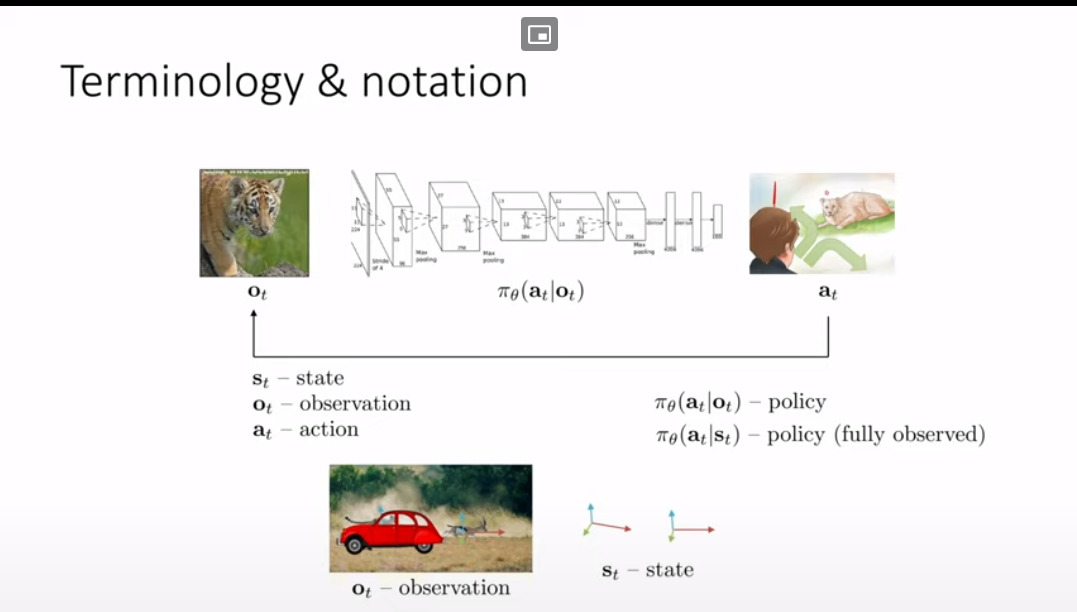
\includegraphics[scale=0.4]{cap2img/slide4.png}
\end{center}
\caption{Representation of state and observation, notations and policy}
\label{fig:cheetah}
\end{figure}

\prettyref{fig:cheetah} shows the state representation of the observation. As we can see, the image shows a car in front
of the cheetah, but the state can represent cheetah using position and vectors. In that case, observation may be
insufficient for the model infers about the cheetah.


\subsection*{Slide 5}%
\label{sub:Slide 5}

\begin{figure}
\begin{center}
    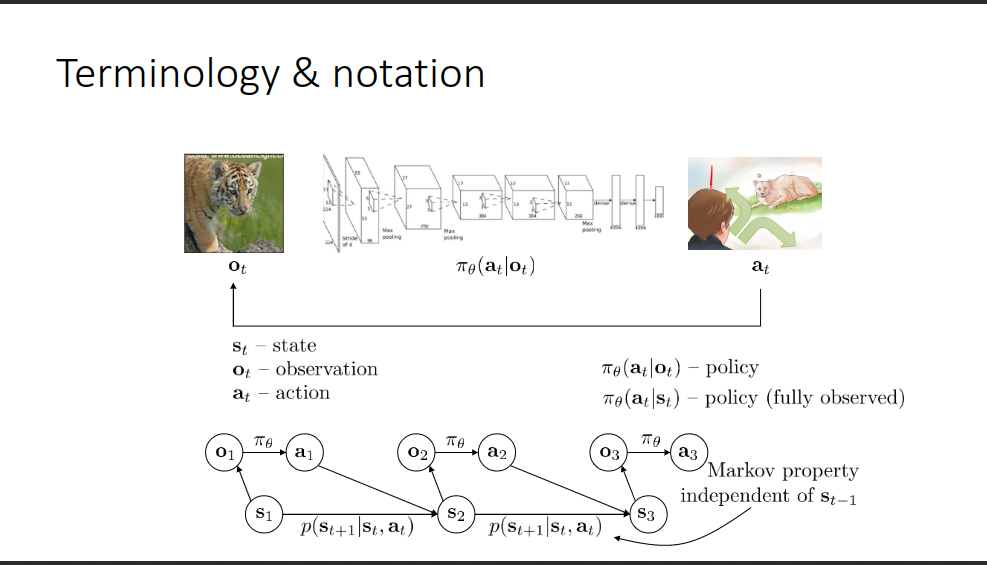
\includegraphics[scale=0.4]{cap2img/slide5.png}
\end{center}
\caption{Markov Chain of the given observation, state and action}
\label{fig:markov}
\end{figure}

\prettyref{fig:markov} has a Markov chain representing each element of the decision-making. $p(s_{t+1}|s_{t},a_{t})$
represents the probability of entering the next state $(s_{t + 1}) $ given the current state and the current
action.

\par  State $s_{3}$ is independent of $s_{1}$ given $s_{2}$ . It uses the \textbf{d-separation} procedure as prof
independence. If you know
the present, then the future is conditionally independent of the past. 
\par If the model only uses the observations and not the states, they do not form a Markov chain. Further,
the observations are not independent among themselves, in such a way that $o_{3} $is not independent of $o_{1} $ given
$o_{2}$.


\subsection*{Slide  7:12 - Imitation Learning}%
\label{sub:Slide 7}

\par \textbf{Behavioral cloning}: Uses the observation state and action to create a training dataset. Using this
training dataset to train the policy is going to result in a bad generalization. 
 The distribution of the training dataset can't cover all situations, so maybe the policy can't deal with
 surprise elements.Also, it does not fit into a markovian model because of the dependence of observation spaces. For
 example, missing images of the car on another lane can struggle with the performance of the model.

\begin{figure}
\begin{center}
    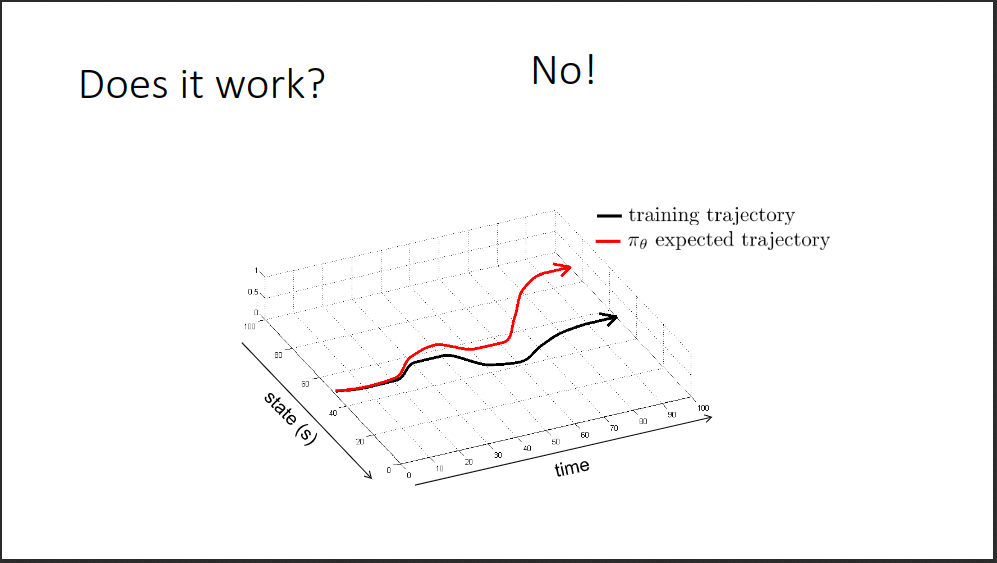
\includegraphics[scale=0.4]{cap2img/slide8.png}
\end{center}
\caption{Sequences of states over time.}
\label{fig:trajectory}
\end{figure}

\par The trajectories demonstrate in \prettyref{fig:trajectory} show that the training trajectory is different from
the expected trajectory. It is because when policy commits a mistake, there is a chance that it is going to a state that it
hasn't seen in the training dataset. Consequently, the model commits another mistake, more significant than the last one. Now the
policy is in state that highly different from the training distribution. Another mistake is going to happen. The mistakes
gradually accumulate through time. AS you can see, the expected trajectory ends up been abruptly different from
the training trajectory. 

\par
Using different trajectories, with some noise, helps the model to recover from smaller mistakes. 
These "erroneous" trajectories create a more robust policy.  However, blind spots problems persist here.

\begin{figure}
\begin{center}
    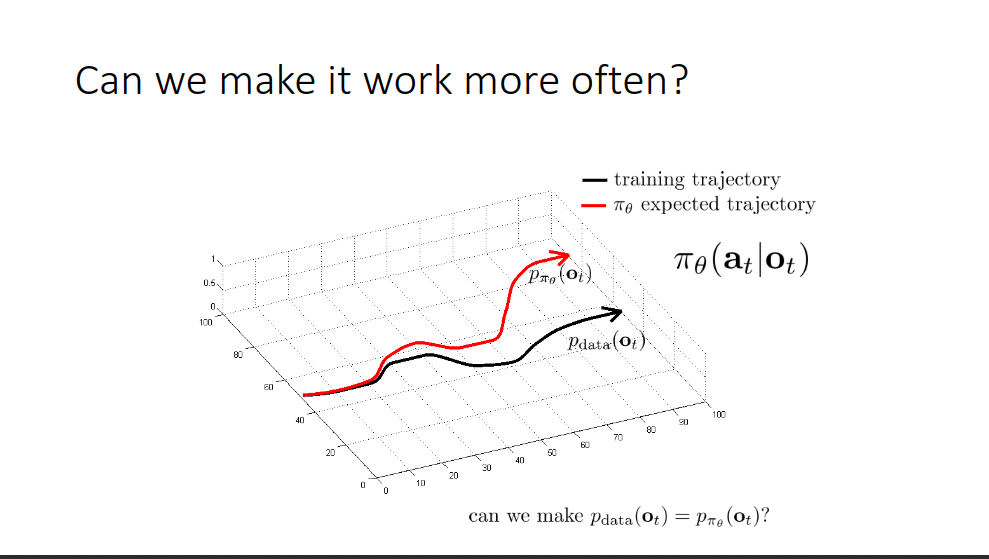
\includegraphics[scale=0.4]{cap2img/slide12.png}
\end{center}
\caption{}
\label{fig:formalization}
\end{figure}

\par \textbf{Mathematical problem formalization}: 
The explanation for the difficulty of training the behavioral cloning model is the drift. 
Once the mode makes the first mistake, the policy starts making more significant mistakes. The observation sampled from training data is
called $p_{data}(o_{t})$.The observations have dependencies among them. But, supervised learning methods disregard these dependencies. 
The policy trained with sampled observations is going to generate actions with mistakes. 
These actions result in observation data also. But, this observation has a different distribution from
$p_{data}(o_t)$. This new distribution is called $p_{\pi_{\theta}}(o_t)$. These two distributions made explicit here
are different because the policy takes different actions. So, how can we make these two distributions, $p_{data} $and
$p_{\pi_\theta}$ , equals and make the imitation learning achieves a reasonable performance? 

\par The questions: Can we make $ p_{data}(o_{t}) = p_{\pi_{\theta}}(o_{t})$? See \prettyref{fig:formalization} to
understand.

\subsection*{Slides 13:16 - DAgger: Dataset Aggregation}%
\label{sub:Slides 13:16 - DAgger: Dataset Aggregation}

\par Goal: Collect training data from $p_{\pi_{\theta}}(o_{t})$  instead of $p_{data}(o_{t})$. How to achieve this?
Just run the policy.

\begin{enumerate}
    \item Train $\pi_{\theta}(a_{t}|o_{t})$  from human data $D $ = \{ $o_{1}, a_{1}, \cdots, o_{n}, a_{n}$ \}
    \item run $\pi_{\theta}(a_{t}|o_{t})$ to get dataset $D_{\pi}$ = \{$o_{1}, \cdots, o_{M}$ \}
    \item Ask human to label $D_{\pi}$ with actions $a_{t}$
    \item Aggregate: $ D \leftarrow D \cup D_{\pi}$
\end{enumerate}

\subsection*{Slide 15}%
\label{sub:Slide 15}

\begin{figure}
\begin{center}
    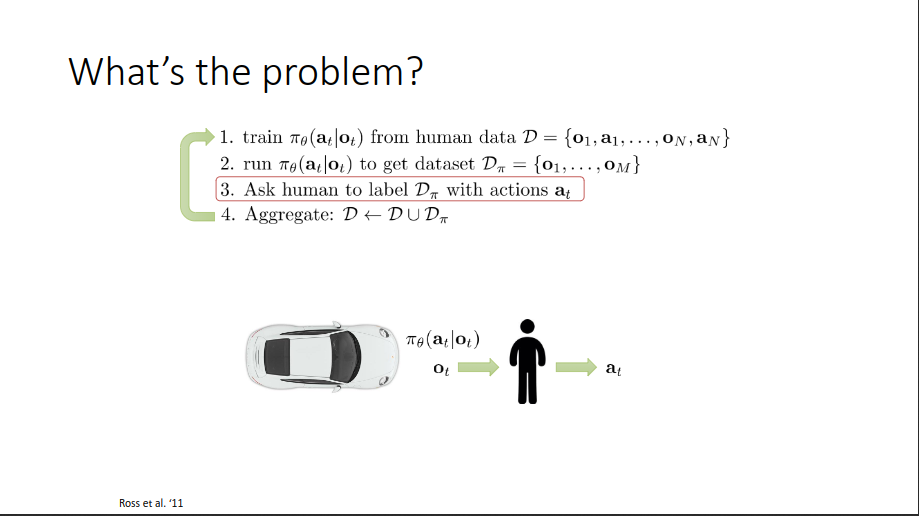
\includegraphics[scale=0.4]{cap2img/slide15.png}
\end{center}
\caption{}
\label{fig:problem_dagger}
\end{figure}


\par What is the problem? Using a human to label the observations is expensive. Also, it is necessary to do it
iteratively as the model train. Another problem is that people might not provide good labels; in that way, the
policy(model) can't achieve reasonable performance.

\subsection*{Slide 16}%
\label{sub:Slide 16}
Can we make Dagger work without more data?
\begin{itemize}
    \item Dagger addresses the problem of distributional "drift". Drift occurs because model makes mistakes,
        creating a different distribution for observations.
    \item Theoretical solution: What if the model is so good that it doesn't make mistakes(drift)?
    \item So, the model must mimic expert behavior very accurately. Is it possible?
    \item Model has to avoid overfitting. 
\end{itemize}


\begin{figure}
\begin{center}
    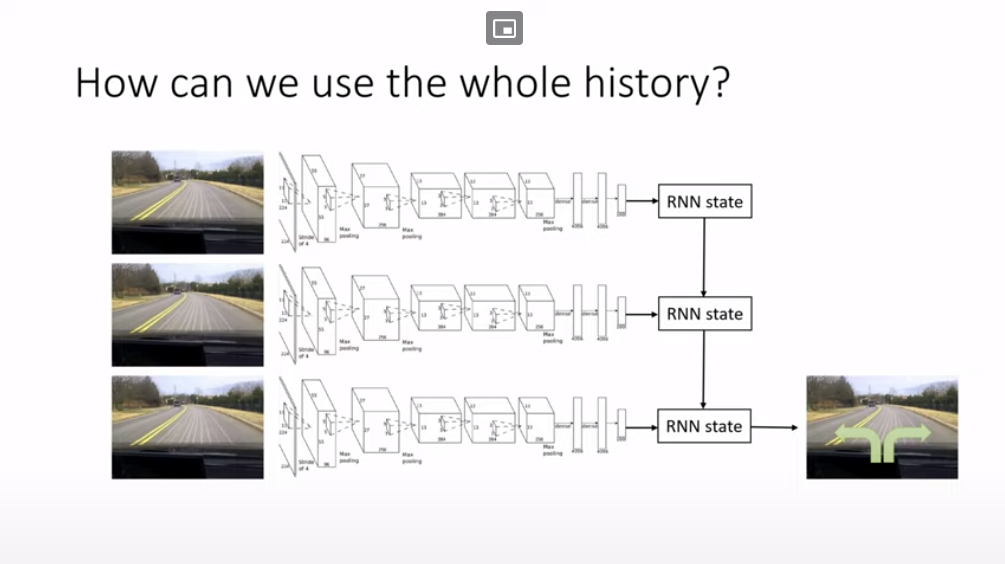
\includegraphics[scale=0.4]{cap2img/slide18.png}
\end{center}
\caption{Recurrent Model}
\label{fig:rnn}
\end{figure}

\subsection*{Slide 17:24 - Problems encountered with DAgger }%
\label{sub:Slide 17}

\begin{figure}[!ht]
\centering
\begin{minipage}[t]{.45\textwidth}
    \centering
    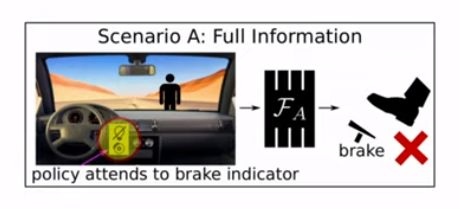
\includegraphics[scale=0.4]{cap2img/slide20a.png}
    \caption{With dashboard}
    \label{fig:breakindicator1}
\end{minipage}
\begin{minipage}[t]{.45\textwidth}
    \centering
    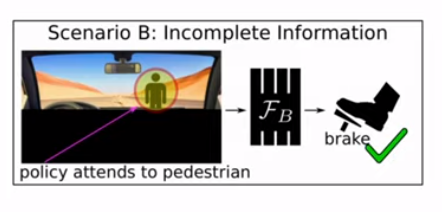
\includegraphics[scale=0.4]{cap2img/slide20b.png}
    \caption{Without dashboard}
    \label{fig:breakindicator2}
\end{minipage}
\label{fig:breakindicatorfig}
\end{figure}

\begin{figure}
\begin{center}
    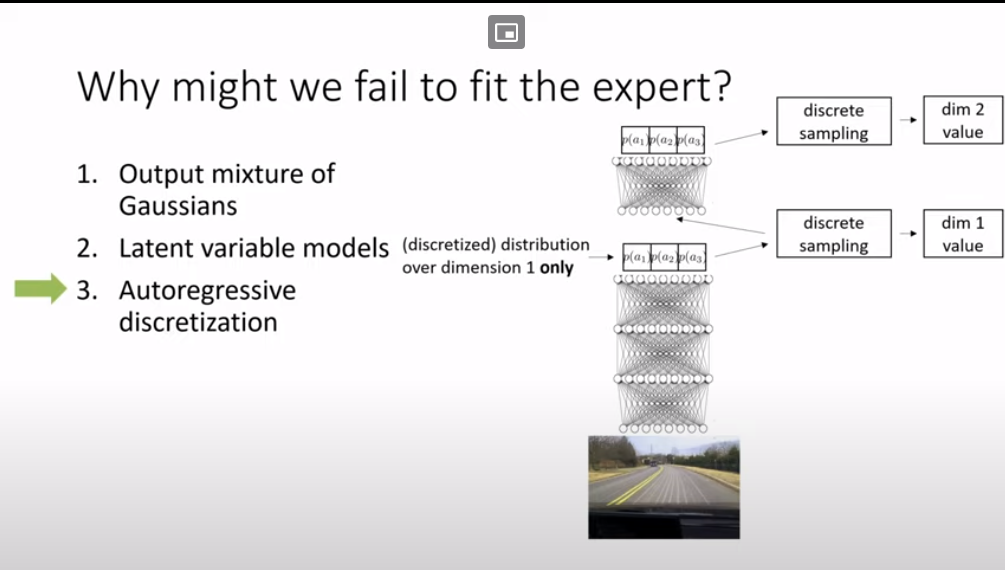
\includegraphics[scale=0.4]{cap2img/slide24.png}
\end{center}
\caption{Autoregressive discretization model demonstrations}
\label{fig:autoregressive}
\end{figure}



\par Why might we fail to fit the expert? Why might the model not mimic the expert's behavior very well?
\begin{enumerate}
    \item Non-Markovian behavior: A policy is a distribution of our actions conditional on the current
        observation. $\pi_{\theta}(a_{t}|o_{t})$ Behavior depends only on current observation. If we see the
        same thing twice, we do the same thing twice, regardless of what happened before. But, it is very
        unnatural for human demonstrators. It is very kind of unnatural for people to act in a truly markovian
        way because we can react in slightly or considerably different ways in the same situation. So a better model
        might be something that produces a distribution over the action condition on a history of past observations
        $\rightarrow \pi_{\theta}(a_{t}|o_{1}, \cdots, o_{t})$. The best model to deal with Non-Markovian observations
        is recurrent models showed in \prettyref{fig:rnn}. 
    \begin{itemize}
        \item RNN is expensive to train and evaluation.
        \item Aside: why might this work poorly? - Causal Confusion - In \prettyref{fig:breakindicator1}
            shows a dashboard with the light on the car's panel. The light indicates the usage of the brake. In that
            case, the model is going to learn that if the light is on then, press the brake, not the other way around.
        \item Aside: why might this work poorly? - Causal Confusion - In \prettyref{fig:breakindicator2} shows a
            scenario without a dashboard.
            However, the model can create correlation with things that happens in the past. Unexpected actions are going
            to happen, breaking far away from the traffic light.
        \item see: Hann et al,. "Causal Confusion in Imitation Learning"
        \item Empirical DAgger can mitigate causal confusion.
    \end{itemize}
    \item Multimodal behavior: Use the average of two good actions. However, the average of good actions can be a lousy action
        instead of a good one. Continuous action is most affected by this problem. Solutions:
    \begin{itemize}
        \item  Output mixture of Gaussians: $\pi(a|o)  = \sum_{i} w_{i}\mathcal{N}(\mu_{i},\Sigma_{i})$ -
            Instead of output the mean and variance of a single normal distribution, output N's different
            normal distributions(mean, variance) and outputs weights on each of the N distributions. This model
            might not work so well if the action space is humongous. But it is straightforward to implement
        \item Latent variable models: Can express complex things, but they are hard to train. Ex: Conditional
            Variational Autoencoder(Explained in the second part of the course), Normalizing flow/realNVP or Stein Variational Gradient Descent.
        \item  Autoregressive discretization: Works in low dimension action space. Using bins to discretize continuous
            actions. It discretizes one dimension at a time and uses softmax into discrete samples. Consequently, it has
            a dim 1 value. Feed it as input into another neural net with the images. The output is another discrete dim 1 value,
            repeat the process. Look at \prettyref{fig:autoregressive}
    \end{itemize}
\end{enumerate}


\subsection*{Slide 29 - Imitation learning: What is the problem?}%
\label{sub:Slide 29}

\begin{itemize}
    \item Humans need to provide data, which is typically finite
        \begin{itemize}
            \item Deep learning works best when data is plentiful
        \end{itemize}
    \item Humans are not good at providing some kinds of actions
    \item Humans can learn autonomously; Can your machines do the same?
    \begin{itemize}
        \item Unlimited data from own experience
        \item Continuous self-improvement
    \end{itemize}
\end{itemize}

\subsection*{Slide 30 - Terminology \& Notation}%
\label{sub:Slide 30 - Terminology_Notation}
\begin{figure}
\begin{center}
    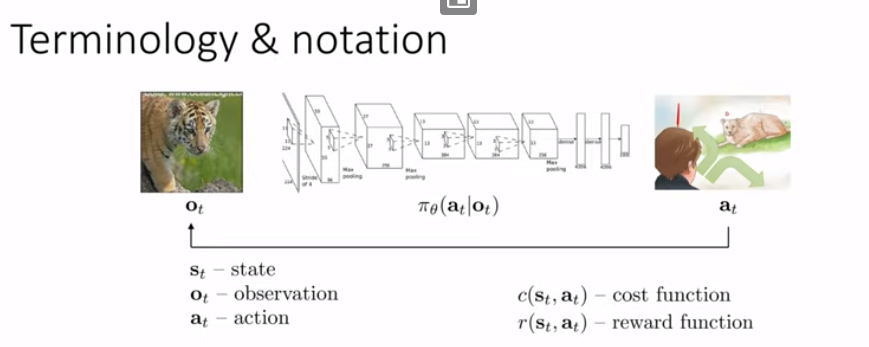
\includegraphics[scale=0.4]{cap2img/slide30.png}
\end{center}
\caption{Terminology \& Notation}
\label{fig:term}
\end{figure}


\par Using a new notation and modify the last terminology a little bit to start thinking about learning without
imitation. \prettyref{fig:term}

\begin{equation}\label{eqn:minimize_1}
    \underset{\theta}{min} E_{a \sim \pi_{\theta}(a|s),s'\sim p(s'|s,a)}[\delta(s' = \text{eaten by tiger})] 
\end{equation}

\begin{equation}\label{eqn:minimize_2}
    \underset{\theta}{min}E_{s_{1:T},a_{1:T}}[\sum_{t} \delta(s_{t} = \text{eaten by tiger})]
\end{equation}

\begin{equation}\label{eqn:minimize_3}
    \underset{\theta}{min}E_{s_{1:T},a_{1:T}}[\sum_{t}c(s_{t},a_{t})]
\end{equation}

Equation \eqref{eqn:minimize_1} means: Minimize the expected number of times the tiger eats someone. Delta
function is one if the tiger eats it or zero otherwise. While equation \eqref{eqn:minimize_2} is minimization
using the temporal aspect.  It minimizes the expectation for a sequence of states and actions of the delta function for
being eaten by the tiger and it is closer to what a proper reinforcement problem seems. Replacing delta function
with cost and then equation \eqref{eqn:minimize_2} transform to equation \eqref{eqn:minimize_3}. Now, we want to minimize these costs over a time
sequence. The distributions of states are according to the dynamics, and the actions distribute according to the policy. The cost gives the model a numerical
quantity of how bad things are, so getting eaten by a tiger might have a cost of a million and get bitten by a mosquito might have a cost of one. The other
option used is the transformation of the cost function into a reward function but as a maximization objective. 

\subsection*{Slide 32 - A cost function for imitation?}%
\label{sub:Slide 32 - A cost function for imitation?}

It is possible to formalize reward and cost function to an imitation model. 
\eqref{eq:costreward}:

\begin{align}
    \label{eq:costreward}
    r(s,a) = logp(a=\pi*(s)|s) && c(s,a) = \Bigg\{ 
        \begin{aligned} 
            & \text{0 if a }= \pi*(s) \\
            & 1 \ \text{otherwise}
        \end{aligned}
\end{align}

\begin{itemize}
    \item Reward function: Maximize the log probability of the policy's action matches the action from deterministic optimal policy $\pi*$
    \item Cost function:  Cost is zero if action matches the optimal action and one otherwise. Zero one loss. Just
        counting the number of mistakes the model makes. Don't care about where the model is in a good state
        or bad state; only care about is whether the model did the same thing as what the expert would have
        done.
\end{itemize}

\subsection*{Analysis}%
\label{sub:Analysis}

Using the cost function from equations \eqref{eq:costreward}. 
Assume:
\begin{equation}
    \label{eq:cost}
    \begin{split}
    \pi_{\theta}(a \neq \pi*(s)|s) \leq \epsilon \\ 
\text{for all s} \in D_{train}
    \end{split}
\end{equation}

\par This assumption in equations \eqref{eq:cost} says: Probability of taking the wrong action would be less than or
equal to $\epsilon$. In other words, it says the model can memorize the data, but no perfectl.The value of $\epsilon$
depends on how good the model is. Better models have small $\epsilon$ . 
\begin{equation}
    \label{eq:sumecost1}
    \mathbb{E} \left[ \sum_{t}c(s_{t},a_{t}) \right] \leq \underbrace{\epsilon t + (1 - \epsilon)(\epsilon (t - 1) + (1
    - \epsilon)(\cdots))}_{\text{T terms, each O($\epsilon $t)}}
\end{equation}



\par Equation \eqref{eq:sumecost1} states: T is the total steps to achieve the objective. $\epsilon \mathbb{T}$$ $ is
the probability off falling off. So once the model makes one mistake, the model just makes mistakes forever. If the model
doesn't fall off, then it has $(1 - \epsilon)$ (that is the probability of not falling off) probability of taking the
right action and go to the next state, which is in its training set and then basically the same thing happens. It
gets the probability $\epsilon (T - 1)$ of falling off to the next T - 1 steps and then repeats. Assuming the $(1 -
\epsilon) $ is close to 1, each of these terms in the sum is on the order of $\epsilon T$. So, it has T terms,
each $O(\epsilon T)$, hence the bound going to be $O(\epsilon T^{2})$. It means that as the length of the time steps
grows, the number of mistakes increases quadratically. Briefly, this assumption is not good because the generalization of
models isn't taking account of this assumption. 


\subsection*{More General Analysis}%
\label{sub:More General Analysis}

\par Using cost function from \eqref{eq:costreward}, let's do a less naive analysis. Assume:
\begin{equation}
    \label{eq:cost2}
    \begin{split}
    \pi_{\theta}(a \neq \pi*(s)|s) \leq \epsilon \\ 
    \text{for \textbf{s} } \sim p_{train}(s)
    \end{split}
\end{equation}
\par States sampled from $p_{train}$ distribution.  For states that were not sampled from this distribution, all bets
are off (It is not possible to say if some sampled is from $p_{data}$ or other distribution). The objective of the
proof is: Even if the samples come from another distribution, it is possible to get samples that look like samples from
$p_{train}$. 

\subsubsection*{Dagger}
With DAgger, $p_{train}(s) \rightarrow p_{\theta}(s)$. The $p_{train} $ distribution converges  to $p_{\theta} $ distribution
whenever the model uses the policy and aggregation operation explained above is used. If $p_{train}  $becomes equal to
$p_{\theta}$  then bound of the expectation of the total cost is  $\epsilon T$. It is assume that the model never end up seeing out of
distribution states because the distributions is equal. Every single step $\epsilon $  probability  to fall off, then
there are T steps.

\begin{equation}
    \mathbb{E} \left[ \sum_{t} c(s_{t},a_{t}) \right] \leq \epsilon T
\end{equation}

\subsubsection*{Behavioral Cloning}
\par If $p_{train} (s)\neq p_{\theta}(s)$:
\begin{equation}
    \label{eq:sumpo}
    p_{\theta}(s_{t}) =\underbrace{(1 - \epsilon)^{t}}_{\mathclap{\text{probability we made no mistakes}}} p_{train}(s_{t})
    +(1 - (1 - \epsilon)^{t})\underbrace{p_{mistake}(s_{t})}_{\mathclap{\text{some other distribution}}}
\end{equation}

\par 
Distribution of states at time step T.  The first term of equation \eqref{eq:sumpo} means the probability of not
making a mistake. The model is at a time step T is indistinguishable from where the expert would have been. The other
part of equation \eqref{eq:sumpo}  is some other distribution we don't know. 

\begin{equation}
    \label{eq:divergence}
    |p_{\theta}(s_{t}) - p_{train}(s_{t})| = (1 - (1 - \epsilon)^{t})|p_{mistake}(s_{t}) - p_{train}(s_{t})|
\end{equation}
\par Equation \eqref{eq:divergence} states the total variation divergence between two distributions.  The maximum
value possible is 2, when two distributions are totally different. 

\begin{equation}
    \label{eq:divergence2}
    |p_{\theta}(s_{t}) - p_{train}(s_{t})| = \sum_{s_{t}}|p_{\theta}(s_{t}) - p_{train}(s_{t})|
\end{equation}

\par  Using the expression after the equal signal from equation \eqref{eq:sumpo} to replace $p_{\theta}$ and $p_{train}$
results in equation \eqref{eq:divergence2}:  

\begin{equation}
    \label{eq:divergence3}
    \begin{split}
    (1 - \epsilon)^{t} p_{train}(s_{t}) + (1 - (1 - \epsilon)^{t})p_{mistake}(s_{t}) \\ 
    - (1 - \epsilon)^{t}    p_{train}(s_{t}) - (1 - (1 - \epsilon)^{t})p_{train}(s_{t}) = \\
    \sum_{s_{t}}|p_{\theta}(s_{t}) - p_{train}(s_{t})|
    \end{split}
\end{equation}

\par Cancels $(1 - \epsilon)^{t}p_{train}(s_{t})$  above in equation \eqref{eq:divergence3}. $(1 -(1 - \epsilon))$ is
positive, putting it in evidence, hence take outside of absolute value. Because of this: 

\begin{equation}
    \label{eq:divergence4}
    |p_{\theta}(s_{t}) - p_{train}(s_{t})| = (1 - (1- \epsilon)^{t}))|p_{mistake}(s_{t}) - p_{train}(s_{t})|
\end{equation}

\par As mentioned before, the worst possible total variation divergence value is 2.  Area of PDF(probability density
function) is 1,  as a consequence, when two distributions are different, and the mass doesn't overlap, the sum
of the area is 2. With this in mind: 

\begin{equation}
    \label{eq:divergence5}
    |p_{\theta}(s_{t}) - p_{train}(s_{t})| = (1 - (1- \epsilon)^{t}))|p_{mistake}(s_{t}) - p_{train}(s_{t})| \leq
    2(1 - (1 - \epsilon)^{t})
\end{equation}

\par Useful identity: $(1 - \epsilon)^{t} \geq 1 - \epsilon t \text{ for } \epsilon \in [0,1]$ =$(1 - (1 -
\epsilon)^{t}) \leq \epsilon t$

\par As result, \eqref{eq:divergence5} is:

\begin{equation}
    \label{eq:divergence6}
    |p_{\theta}(s_{t}) - p_{train}(s_{t})| = (1 - (1- \epsilon)^{t}))|p_{mistake}(s_{t}) - p_{train}(s_{t})| \leq
    2\epsilon t
\end{equation}

\par Using equation \eqref{eq:divergence6}  and calculate the bound of the cost.  Pushing expectation inside the
sum by the linearity of expectation: 

\begin{equation}
    \label{eq:costbound}
        \sum_{t}\mathbb{E}_{p\theta(s_{t})}[c_{t}] = \sum_{t} \sum_{s_{t}} p_{\theta}(s_{t})c_{t}(s_{t}) \leq
    \sum_{t}\sum_{s_{t}} p_{train}(s_{t})c_{t}(s_{t}) + |p_{\theta}(s_{t}) - p_{train}(s_{t})|c_{max}
\end{equation}

\par Explaining the right part of inequality \eqref{eq:costbound} above:

\begin{equation*}
\begin{aligned}
    p_{\theta} = p_{train} + p_{\theta} - p_{train} \\ 
    p_{\theta}c = p_{train}c + (p_{\theta} - p_{train})c \\ 
    \leq  p_{train}c + |p_{\theta} - p_{train}|c_{max} \\ 
    \text{Adding cost on all terms} \\ 
    \text{When the equation has a difference between two terms} \\
    \text{we know that is less than or equal to the absolute value of difference} \\
    \text{$c_{max} $ is one, because it is a zero-one loss} \\
\end{aligned}
\end{equation*}

\par Returning to equation \eqref{eq:costbound}, now we have all elements for deriving its bound.The single-step of the
first term of the right part of inequality is bounded by $\epsilon$ . Next, the second term, the absolute value, is bounded
by $\epsilon t$ calculated in equation \eqref{eq:divergence6}. 
\begin{equation}
    \sum_{t}\mathbb{E}_{p\theta(s_{t})}[c_{t}] = \sum_{t} \sum_{s_{t}} p_{\theta}(s_{t})c_{t}(s_{t}) \leq \sum_{t}\epsilon +
    2\epsilon t \leq eT + 2\epsilon T^{2}
\end{equation}

\par Using O notation on the bound: $O(\epsilon T^{2})$. It shows why behavioral cloning can be problematic. 



\end{document}

